\documentclass[a4paper,10pt]{book}
\usepackage[bottom=20mm,top=20mm,left=20mm,right=20mm]{geometry}

%-----------------------package---------------------------
\usepackage{amssymb}
\usepackage{amsthm}
\usepackage{bm}
\usepackage{booktabs}
\usepackage{braket}
\usepackage{cancel}
\usepackage{xcolor}
\usepackage{graphicx}
\usepackage{epstopdf}
\usepackage{enumerate}
\usepackage[perpage]{footmisc}
\usepackage[colorlinks=true,linkcolor=blue,citecolor=red,urlcolor=blue,linktocpage=true,breaklinks=true]{hyperref}
\usepackage{mathtools}
\usepackage{subcaption}
\usepackage{times}
\usepackage{tikz}
\usepackage{titlesec}
\usepackage[colorinlistoftodos]{todonotes}
\usepackage{verbatim}
\usetikzlibrary{quantikz2}
\usetikzlibrary{3d}

%-----------------------settings---------------------------
\allowdisplaybreaks[3]
\newtheorem{theorem}{Theorem}[section]
\newtheorem{lemma}{Lemma}[section]
\newtheorem{corollary}[theorem]{Corollary}
\numberwithin{equation}{section}

%-----------------------main text---------------------------
\begin{document}
%coverpage
\begin{titlepage}
    \thispagestyle{empty}
    \vspace*{\fill}
    \begin{center}
        \normalfont
        \LARGE\textbf{Notes on Quantum Search Algorithm}

        \bigskip
        \large{Zhongwei Jiang, Linfeng Zhao}

        \bigskip
        {\href{https://github.com/little-little-red/NoteForQuantumSearchAlgorithm}{Project Link: https://github.com/little-little-red/NoteForQuantumSearchAlgorithm}}

        \bigskip
        \normalsize{\today}
    \end{center}
    \vspace*{\fill}
    \newpage
\end{titlepage}
%contentspage
\pagenumbering{Roman}
\tableofcontents
\newpage
%maintext
\pagenumbering{arabic}
\chapter{Quantum Computation}

\textit{This chapter is based on the book\cite{nielsen2010}.}

\section{Quantum Gate}

\subsection{Single-qubit gate}

The number of qubits in a quantum state depends on the number of classical bits in its dimension, so we usually call a vector $\ket{\psi} = a\ket{0} + b\ket{1}$ parameterized by two complex numbers $a$ and $b$ satisfying $|a|^2 + |b|^2 = 1$ a qubit. According to the constraints and phase redundancy, the Bloch sphere representation gives us a more intuitive way to observe the qubit, an isomorphism from a qubit to the three-dimensional real sphere:
\begin{equation}\label{BlochSphereRepersentation}
    \begin{split}
        \mathbb{C}\mathbb{P}^{1}                                                                              & \to S^{2}                                                                            \\
        \ket{\psi} = \cos \frac{\theta}{2}\ket{0} + \mathrm{e}^{\mathrm{i}\varphi}\sin\frac{\theta}{2}\ket{1} & \mapsto \vec{n}_{\psi}=(\cos\varphi\sin\theta,\sin\varphi\sin\theta,\cos\theta)^{T}.
    \end{split}
\end{equation}
where $\theta\in\left[0,\pi\right]$ and $\varphi\in\left[0,2\pi\right]$.

Operations on a qubit must preserve the norm and thus are described by $2\times2$ unitary matrices. By $\det|U|=e^{2i\alpha}$ Then
\begin{equation}
    e^{-i\alpha}U\in SU(2)
\end{equation}
They're only off by one global phase, so we usually ignore the global phase and only consider $SU(2)$. The Lie group $SU(2)$ has three generators $i\sigma_j$, $\sigma_j$ called Pauli matrices:
\begin{equation}
    \sigma_x = \begin{pmatrix} 0 & 1 \\ 1 & 0 \end{pmatrix}, \quad
    \sigma_y = \begin{pmatrix} 0 & -i \\ i & 0 \end{pmatrix}, \quad
    \sigma_z = \begin{pmatrix} 1 & 0 \\ 0 & -1 \end{pmatrix}.
\end{equation}
From Lie group elements, any single-qubit unitary can be written as a product of exponentials of Pauli matrices by a global phase:
\begin{equation}
    U = e^{i\alpha}\exp\left(-i\frac{\omega}{2}\vec{n}\cdot\vec{\sigma}\right),
\end{equation}
which $\vec{n}$ is the coordinates of the rotation axis on the Bloch sphere.
From the isomorphism \ref{BlochSphereRepersentation}, we can also induce an isomorphism of operations on two spaces:
\begin{equation}
    \begin{split}
        SU(2)/\{\pm 1\}                                             & \to SO(3)
        \\
        \exp\left(-i\frac{\omega}{2}\vec{n}\cdot\vec{\sigma}\right) & \mapsto \exp\left(\omega\vec{n}\cdot\vec{J}\right)
    \end{split}
\end{equation}
which $\omega\in\left[0,\pi\right]$ and $J_{j}$ are the three generators of Lie group $SO(3)$, the former refers to single-qubit gates and the latter to transformations on the Bloch sphere. For visualization and convenience, we let $R_{\vec{n}}(\omega) \coloneqq \exp\left(-i\frac{\omega}{2}\vec{n}\cdot\vec{\sigma}\right)$.

In the following, we use $XYZ$ instead of $\sigma_x\sigma_y\sigma_z$, here are some other single-qubit gates which are frequently used, they are called Hadamard gate, phase gate, and $\pi/8$ gate:
\begin{equation}
    H = \frac{1}{\sqrt{2}}\begin{pmatrix} 1 & 1 \\ 1 & -1 \end{pmatrix}, \quad
    S = \begin{pmatrix} 1 & 0 \\ 0 & i \end{pmatrix}, \quad
    T = \begin{pmatrix} 1 & 0 \\ 0 & e^{i\pi/4} \end{pmatrix}.
\end{equation}



\subsection{Properties of single-qubit gate}

Here we list some properties of single-qubit gates:
\begin{theorem}\label{the:EulerAngle}
    A single qubit gate $U$ can be decomposed into the following form
    \begin{equation}
        U=e^{i\alpha}R_{z}(\beta)R_{y}(\gamma)R_{z}(\delta).
    \end{equation}
\end{theorem}
\begin{corollary}\label{cor:DecompositionByTwoAxis}
    For suitable parameters $\alpha$, $\beta_{k}$, $\gamma_{k}$ and nonparallel vectors $\vec{n}$ and $\vec{m}$, there is
    \begin{equation}
        U=e^{i\alpha}\prod_{j=1}^{k}R_{\vec{n}}(\beta_{j})R_{\vec{m}}(\gamma_{j}).
    \end{equation}
\end{corollary}
\begin{corollary}\label{DecToAXBXC}
    If $U$ is a single qubit gate, then there exists $A,B,C \in SU(2)$, $ABC=I$, and then there is
    \begin{equation}
        U = e^{i\alpha}AXBXC
    \end{equation}
\end{corollary}
\begin{proof}
    let
    \begin{equation*}
        A=R_{z}(\beta)R_{y}(\gamma/2),\ B=R_{y}(-\gamma/2)R_{z}(-(\gamma+\beta)/2),\ C=R_{z}((\gamma-\beta)/2)
    \end{equation*}
    then we have
    \begin{equation}
        AXBXC=R_{z}(\beta)R_{y}(\gamma)R_{z}(\delta)
    \end{equation}
    and $ABC=I$.
\end{proof}
\begin{theorem}\label{ProductOfPauli}
    We have the product of Pauli matrices,
    \begin{equation}
        \sigma_{j}\sigma_{k} = i\epsilon_{jk}^{l}\sigma_{l}+\delta_{jk}I.
    \end{equation}
\end{theorem}
\begin{corollary}\label{cor:CompositionOfRotation}
    The element of Lie group $SU(2)$ can be changed into the following form,
    \begin{equation}
        R_{\vec{n}}(\omega) \coloneqq \exp\left(-i\frac{\omega}{2}\vec{n}\cdot\vec{\sigma}\right)=\cos \left(\frac{\omega}{2}\right)I-i\sin \left(\frac{\omega}{2}\right)(\vec{n}\cdot\vec{\sigma}).
    \end{equation}
\end{corollary}
\begin{proof}
    Considering the Taylor expansion
    \begin{equation}
        \begin{split}
            \exp\left(-i\frac{\omega}{2}\vec{n}\cdot\vec{\sigma}\right)
             & = \sum_{k=0}^{\infty}\frac{1}{k!}\left(-i\frac{\omega}{2}\vec{n}\cdot\vec{\sigma}\right)^{k}                                                                                                                          \\
             & = \sum_{k=0}^{\infty}\frac{1}{(2k)!}\left(-i\frac{\omega}{2}\right)^{2k}(\vec{n}\cdot\vec{\sigma})^{2k} + \sum_{k=0}^{\infty}\frac{1}{(2k+1)!}\left(-i\frac{\omega}{2}\right)^{2k+1}(\vec{n}\cdot\vec{\sigma})^{2k+1} \\
             & = \cos \left(\frac{\omega}{2}\right)I-i\sin \left(\frac{\omega}{2}\right)(\vec{n}\cdot\vec{\sigma}),
        \end{split}
    \end{equation}
    where we have $(\vec{n}\cdot\vec{\sigma})^{2} = I$ from the theorem \ref{ProductOfPauli}.
\end{proof}
\begin{corollary}
    If a rotation through an angle $2\omega_{1}$ about an axis $\vec{n_{1}}$ is followed by a rotation through an angle $2\omega_{2}$ about an axis $\vec{n_{2}}$, then the overall rotation is through an angle $\omega_{12}$ about an axis $\vec{n_{12}}$ given by
    \begin{equation*}
        \begin{split}
            \cos\omega_{12}             & = \cos\omega_{1}\cos\omega_{2}-\sin\omega_{1}\sin\omega_{2}\vec{n_{1}}\cdot\vec{n_{2}}                                                      \\
            \sin\omega_{12}\vec{n_{12}} & = \sin\omega_{1}\cos\omega_{2}\vec{n_{2}}+\cos\omega_{1}\sin\omega_{2}\vec{n_{2}}+\sin\omega_{1}\sin\omega_{2}\vec{n_{1}}\times\vec{n_{2}}.
        \end{split}
    \end{equation*}
\end{corollary}
\begin{proof}
    We know $R_{\vec{n_{1}}}(2\omega_{1})=\cos\omega I-i\sin\omega(\vec{n_{1}}\cdot\vec{\sigma})$ and the same as index $2$, so the product of two rotations is
    \begin{equation*}
        \begin{split}
              & R_{\vec{n_{1}}}(2\omega_{1})R_{\vec{n_{2}}}(2\omega_{2})                                                                                                                                                                                       \\
            = & \cos\omega_{1}\cos\omega_{2}I-i\sin\omega_{1}\cos\omega_{2}(\vec{n_{1}}\cdot\vec{\sigma})-i\cos\omega_{1}\sin\omega_{2}(\vec{n_{2}}\cdot\vec{\sigma})-\sin\omega_{1}\sin\omega_{2}(\vec{n_{1}}\cdot\vec{\sigma})(\vec{n_{2}}\cdot\vec{\sigma}) \\
            = & \cos\omega_{12}I-i\sin\omega_{12}(\vec{n_{12}}\cdot\vec{\sigma}),
        \end{split}
    \end{equation*}
    where we have $(\vec{n_{1}}\cdot\vec{\sigma})(\vec{n_{2}}\cdot\vec{\sigma})=i(\vec{n_{1}}\times\vec{n_{2}})\cdot\vec{\sigma}+(\vec{n_{1}}\cdot\vec{n_{2}})\cdot\vec{\sigma}$ from Theorem \ref{ProductOfPauli}.
\end{proof}



\subsection{\label{CtrlGate}Controlled operation}

Analogous to the if statement of a classical circuit, we can use the controlled-NOT gate to control the target qubit with the control qubit, its matrix form and circuit are shown as follows:
\begin{equation}
    CNOT = \begin{pmatrix} I & 0 \\ 0 & X \end{pmatrix}
\end{equation}
\begin{equation}
    \begin{quantikz}[row sep=0.4cm]
        & \ctrl{1} & \\
        & \targ{} &
    \end{quantikz}
\end{equation}
CNOT gate makes the state of the target qubit be flipped when the control qubit is 1 and remains unchanged when the control qubit is 0. That is $\ket{c}\ket{t}\rightarrow\ket{c}X^{c}\ket{t}$. We will also use two deformations of CNOT gates:
\begin{equation}
    \begin{quantikz}
        & \targ{} & \ghost{H} \\
        & \ctrl{-1} & \ghost{H}
    \end{quantikz} = \begin{quantikz}[row sep=0.4cm,column sep=0.4cm]
        & \gate{H} & \ctrl{1} & \gate{H} & \\
        & \gate{H} & \targ{} & \gate{H} &
    \end{quantikz}
    \quad\text{and}\quad
    \begin{quantikz}
        & \octrl{1} & \ghost{X} \\
        & \targ{} &
    \end{quantikz} = \begin{quantikz}[row sep=0.4cm,column sep=0.4cm]
        & \gate{X} & \ctrl{1} & \gate{X} & \\
        & & \targ{} & &
    \end{quantikz}
\end{equation}

We expect to extend this control from $X$ to an arbitrary single-qubit gate $U$. That is, $\ket{c}\ket{t}\rightarrow\ket{c}U^{c}\ket{t}$ which is known as a controlled-U gate. Show that:
\begin{equation}
    \begin{quantikz}[row sep=0.4cm]
        & \ctrl{1} & \\
        & \gate{U} &
    \end{quantikz}
\end{equation}
We wish to decompose this into combining single quantum bit gates and CNOT gates. With the theorem\ref{DecToAXBXC}, we can divide the controlled-U gate into several parts, looking first at the global phase part, which has:
\begin{equation}
    \begin{quantikz}[row sep=0.4cm]
        & \ctrl{1} & \ghost{phase} \\
        & \gate{e^{i\alpha}I} &
    \end{quantikz} = \begin{quantikz}[row sep=0.4cm]
        & \gate{phase} & \\
        & \ghost{e^{i\alpha}I} &
    \end{quantikz}
\end{equation}
where $phase = \begin{pmatrix} 1 & 0 \\ 0 & e^{i\alpha} \end{pmatrix}$.

Looking at the $AXBXC$ part again, we have the expectation that if the control qubit is $\ket{0}$, then we do nothing, and adding a CNOT gate anywhere doesn't change that, so we have.
\begin{equation}
    \begin{quantikz}
        \lstick{$\ket{0}$} & & \ghost{} \\
        \lstick{} & \gate{I} &
    \end{quantikz} = \begin{quantikz}
        & & & & \ghost{} \\
        & \gate{A} & \gate{B} & \gate{C} &
    \end{quantikz} = \begin{quantikz}
        & & \ctrl{1} & & \ctrl{1} & & \ghost{} \\
        & \gate{A} & \targ{} & \gate{B} & \targ{} & \gate{C} &
    \end{quantikz}
\end{equation}
This construction also satisfies: if the control qubit is $\ket{1}$, we apply $AXBXC$ to the target qubit.

So we have that:
\begin{theorem}
    The controlled-U gate can be decomposed with CNOT gates and single-qubit gates into this form:
    \begin{equation}
        \begin{quantikz}
            & \ctrl{1} & \ghost{X} \\
            & \gate{U} &
        \end{quantikz} = \begin{quantikz}
            & & \ctrl{1} & & \ctrl{1} & \gate{phase} & \\
            & \gate{A} & \targ{} & \gate{B} & \targ{} & \gate{C} &
        \end{quantikz}
    \end{equation}
\end{theorem}

Considering the case of multiple control qubits, first look at the case of two control qubits, you can construct: if $V$ is a single qubit gate satisfying $V^2=U$, we have:
\begin{equation}
    \begin{quantikz}
        & \ctrl{1} & \ghost{} \\
        & \ctrl{1} & \ghost{} \\
        & \gate{U} & \qw
    \end{quantikz} = \begin{quantikz}[row sep=0.5cm,column sep=0.4cm]
        & \qw & \ctrl{1} & \qw & \ctrl{1} & \ctrl{2} & \ghost{} \\
        & \ctrl{1} & \targ{} & \ctrl{1} & \targ{} & \qw & \ghost{} \\
        & \gate{V} & \qw & \gate{V^\dagger} & \qw & \gate{V} & \qw
    \end{quantikz}
\end{equation}

Then we can extend this to the case of $n$ control qubits, there are many kinds of construction methods, and we use the recursive method to construct:
\begin{equation}
    \begin{quantikz}[row sep=0.3cm]
        & \ctrl{1} & \ghost{} \\
        & \ctrl{1} & \ghost{} \\
        & \ctrl{1} & \ghost{} \\
        & \gate{U} & \qw
    \end{quantikz} = \begin{quantikz}[row sep=0.3cm,column sep=0.4cm]
        & \qw & \ctrl{1} & \qw & \ctrl{1} & \ctrl{2} & \ghost{} \\
        & \qw & \ctrl{1} & \qw & \ctrl{1} & \ctrl{2} & \ghost{} \\
        & \ctrl{1} & \targ{} & \ctrl{1} & \targ{} & \qw & \ghost{} \\
        & \gate{V} & \qw & \gate{V^\dagger} & \qw & \gate{V} & \qw
    \end{quantikz}
\end{equation}

Ultimately we will show that any unitary operation can be composed to an arbitrarily good approximation from just H, S, T, CNOT gates. Here is the construction of the Toffoli Gate:
\begin{equation}
    \begin{quantikz}[row sep=0.4cm]
        & \ctrl{1} & \ghost{} \\
        & \ctrl{1} & \ghost{} \\
        & \targ{} & \qw
    \end{quantikz} = \begin{quantikz}[row sep=0.15cm,column sep=0.25cm]
        & & & & \ctrl{2} & & & & \ctrl{2} & & \ctrl{1} & & \ctrl{1} & \gate{T} & \\
        & & \ctrl{1} & & & & \ctrl{1} & & & \gate{T^\dagger} & \targ{} & \gate{T^\dagger} & \targ{} & \gate{S} & \\
        & \gate{H} & \targ{}  & \gate{T^\dagger} & \targ{} & \gate{T} & \targ{} & \gate{T^\dagger} & \targ{} & \gate{T} & \gate{H} & & & &
    \end{quantikz}
\end{equation}



\section{Universal Gate Set}

\subsection{\label{subsec:SingleAndCnot}Single-qubit and CNOT gates are universal}

In the section \ref{CtrlGate}, we showed that $C^{n}(U)$ gate can be decomposed into a combination of single-qubit gates and CNOT gates. In this section \ref{subsec:SingleAndCnot}, we will show that any unitary gate can be combined from $C^{n}(U)$ gate.

First, we introduce the lemma:
\begin{lemma}
    Any D-dimensional unitary transformation U can always be decomposed into the product of $d(d-1)/2$ two-level unitary transformations under a natural basis.
\end{lemma}
So exists two-level unitary transformations $ V_{j} $ made $U = \prod\limits_{j=1}^{d(d-1)/2}V_{j}$\footnote{Unless otherwise specified, the conjunction sign in this document is calculated according to the composite order of the map, that is $\prod\limits_{j=1}^{n}a_{j} = a_{n}a_{n-1}\cdots a_{1}$. }. Two-level unitary transformations are unitary matrices that act non-trivially only on two or fewer vector components. The proof idea of this theorem is simple \footnote{Each single-qubit gates has $d(d-1)/2$ degrees of freedom and each two-level unitary transformation turn one of single-qubit gate elements into zero in order. So exists two-level unitary transformations $ V_{j} $ made $\left( \prod\limits_{j=1}^{d(d-1)/2}V_{j} \right) U = I $. },  let's focus on the two-level unitary transformations $V$.

Consider the binary expansion of the two bases $\ket{s}$ and $\ket{t}$ on which $V$ operates, where $s=s_{1}\ldots s_{n}$ and $t=t_{1}\ldots t_{n}$. We can use Toffoli gate to turn $s_{j}$ into $t_{j}$, after $n-1$ steps $\ket{s_{1}\ldots s_{k-1} s_{k} s_{k+1} \ldots s_{n}}$ into $\ket{t_{1}\ldots t_{k-1} s_{k} t_{k+1} \ldots t_{n}}$. It puts $\ket{s}$ and $\ket{t}$in the same qubit and makes $V$ into a $C^{n}(\widetilde{V})$ gate which $\widetilde{V}$ is the non-trivial $2\times 2$ unitary sub-matrix of $V$.

Let's take an example to illustrate this lemma, consider the $U$ gate:
\begin{equation}
    V = \begin{pmatrix} a & 0 & 0 & c \\ 0 & 1 & 0 & 0 \\ 0 & 0 & 1 & 0 \\ b & 0 & 0 & d \end{pmatrix}
    \quad \text{and} \quad
    \widetilde{V} = \begin{pmatrix} a & c \\ b & d \end{pmatrix}
\end{equation}
Notice that $V$ acts non-trivially only on the states $\ket{00}$ and $\ket{11}$, so we can use the CNOT gate to turn $\ket{00}$ into $\ket{01}$, then we can get the $C(\widetilde{V})$ gate. Here is the circuit of $V$:
\begin{equation}
    \begin{quantikz}
        & \gate[2]{V} & \qw \\
        & & \qw
    \end{quantikz} = \begin{quantikz}
        & \octrl{1} & \gate{\widetilde{V}} & \octrl{1} & \qw \\
        & \targ{} & \ctrl{-1} & \targ{} & \qw
    \end{quantikz}
\end{equation}

So we have:
\begin{theorem}
    Any unitary gate can be combined from single-qubit gates and CNOT gates.
\end{theorem}



\subsection{Approximate universal operators with a discrete set}

It is hard to implement all single-qubit gates, so we consider approximating it with a discrete set that we can implement. We introduce the induced norm of operators to measure the degree of approximation:
\begin{equation}
    E(U,V) = \left\| U-V \right\| \coloneqq \sup\limits_{\substack{\ket{\psi} \in \mathbb{C}^{n} \\ \left\| \ket{\psi} \right\| = 1}} \left\| (U-V)\ket{\psi} \right\|
\end{equation}
Where $U$ is the target unitary operator that we wish to implement, $V$ is the unitary operator that is implemented in practice, and $E(U,V)$ is the error when $V$ is implemented instead of $U$. It is natural that:
\begin{theorem}
    In the approximation of $m$ gates, the error is added at most linearly:
    \begin{equation}
        E\left(\prod\limits_{j=1}^{m}U_{j},\prod\limits_{j=1}^{m}V_{j}\right) \leq \sum_{j=1}^{m} E(U_{j},V_{j})
    \end{equation}
\end{theorem}
\begin{proof}
    Considering $\ket{\psi_{0}}$ which maximizes $\left\|\left(\prod\limits_{i=1}^{m}U_{i} -  \prod\limits_{i=1}^{m}V_{i}\right)\ket{\psi}\right\|$ and definition $\ket{\psi_{i}} = V_{i}\ket{\psi_{i-1}}$ , $\ket{\Delta_{i}} = U_{i}\ket{\psi_{i-1}} - \ket{\psi_{i}}$ , we can see that
    \begin{equation*}
        E\left(\prod_{j=1}^{m}U_{j},\prod\limits_{j=1}^{m}V_{j}\right) = \left\|\ket{\Delta_{m}} + \sum\limits_{j=1}^{m-1} \left(\prod_{k=j+1}^{m}U_{k}\right)\ket{\Delta_{j}}\right\| \leq \sum\limits_{j=1}^{m} \left\|\ket{\Delta_{j}}\right\| \leq \sum_{j=1}^{m} E(U_{j},V_{j}) \qedhere
    \end{equation*}
\end{proof}


We are more concerned with the error of the approximation in the measurement. Considering $M$ is a POVM element in an arbitrary measurement POVM, and $P_{U}$(or $P_{V}$) is the probability of obtaining this outcome if $U$(or $V$) were performed with the state $\ket{\psi}$, We can prove\footnote{Let $\ket{\Delta} = (U-V)\ket{\psi}$, notice that $\bra{\psi}U^{\dagger}MU\ket{\psi} - \bra{\psi}V^{\dagger}MV\ket{\psi} = \bra{\psi}U^{\dagger}M\ket{\Delta} + \bra{\Delta}MV\ket{\psi}$. } that:
\begin{equation}
    \left| P_{U} - P_{V} \right| \leq 2E(U,V)
\end{equation}
This makes it possible that if we want the probability difference between the approximate line and the ideal line on a certain outcome to be within a tolerance $\Delta > 0$, we only need to ensure that $E(U_{j},V_{j}) \leq \Delta/(2m)$.

From the decomposition given by corollary \ref{cor:DecompositionByTwoAxis}, we can further care about the degree of approximation of $R_{\vec{n}}(\omega)$. Let's start by introducing a neat lemma :
\begin{lemma}\label{AngleCoverR}
    Considering $\alpha$, $\omega \in \mathbb{R} /2\pi\mathbb{Z}$, if $\omega/\pi \in \mathbb{R} \backslash \mathbb{Q}$ , we can find a sub-sequences $\{x_n\}$ of sequences $\{n\}$ makes $\lim\limits_{n\to\infty}x_n\omega = \alpha$.
\end{lemma}
\begin{proof}
    $\forall \epsilon>0$, $\exists N=\frac{2\pi}{\epsilon}$, when $n>N$, we can find $|j\omega-k\omega|\leq\frac{2\pi}{n}$ which $j,k \in \{n\},j>k$, let $x_{n} = (j-k)\left\lfloor\frac{\alpha}{|j\omega-k\omega|}\right\rfloor$, so we have $|x_{n}\omega-\alpha|<|j\omega-k\omega|\leq\frac{2\pi}{n}<\epsilon$.
\end{proof}
Further, we have\footnote{The construction of $x_{n}$ in this part is only to prove the existence, without considering the complexity. There are far less complex constructs.}:
\begin{equation}
    \begin{split}
          & \ E(R_{\vec{n}}(\alpha),R_{\vec{n}}(\omega)^{x_{n}})              \\
        = & \ E(R_{\vec{n}}(\alpha),R_{\vec{n}}(\alpha+(x_{n}\omega-\alpha))) \\
        = & \ |1-\exp((x_{n}\omega-\alpha)/2)|\leq\ \epsilon/2
    \end{split}
\end{equation}
According to the proof, we just need to find the gate that has the Angle that the theorem requires. Fortunately, the $THTH$ gate has the angel we need. It is a rotation of the Bloch sphere about an axis along $\vec{n} = (\cos\frac{\pi}{8},\sin\frac{\pi}{8},\cos\frac{\pi}{8})$ and through an angle $\omega$ defined by $\cos\frac{\omega}{2} = \cos^{2}\frac{\pi}{8}$, so we just let $R_{\vec{n}}(\omega) = THTH$.

From corollary \ref{cor:DecompositionByTwoAxis}, to construct unitary operator $U$, we still need to approximate the rotation of the other axis, but even more fortunate is that $HR_{\vec{n}}(\omega)H$ is exactly what we need, has axis $\vec{m} = (\cos\frac{\pi}{8},-\sin\frac{\pi}{8},\cos\frac{\pi}{8})$ and the angle $\omega$, like $R_{\vec{n}}(\omega)$, is an irrational multiple of $\pi$. After layers and layers of preparation, let's list the final approximation with suitable positive integers $j_{n}$ to U:
\begin{equation}\label{FinalApproximation}
    E(U,\prod_{j=1}^{2k}R_{\vec{n}}(\omega)^{j_{n}}H) \leq k\epsilon
\end{equation}
\begin{theorem}
    Given any single qubit unitary operator $U$ and any $\epsilon > 0$, it is possible to approximate $U$ to within $\epsilon$ \footnote{The difference between Equation \ref{FinalApproximation} and here by one coefficient can be solved by the setting of $\epsilon$ in the proof of Theorem \ref{AngleCoverR}, but it does not matter. }using a circuit composed of $H$ gates and $T$ gates alone.
\end{theorem}



\subsection{Circuit size for approximation}

It makes no sense to talk about its existence without giving its size,  so let's estimate the number of gates needed for the approximation in the previous section. For convenience of stating the theorem, we say that $S$ is an $\epsilon$-net in $W$, if every point in $W$ is within a distance $\epsilon$ of some point in $S$, where $S$, $W\in SU(2)$ and $\epsilon>0$ and the distance is $D(U,V)\coloneqq\mathrm{tr}|U-V|$. And we define $\mathcal{G}_{l}$ to be the set of all words of length at most $l$.
\begin{theorem}[Solovay-Kitaev theorem]
    Let $\mathcal{G}$ be a finite set of elements in $SU(2)$ containing its own inverses, such that $\left\langle\mathcal{G}\right\rangle$ is dense in $SU(2)$. Let $\epsilon > 0$ be given. Then $\mathcal{G}_{l}$ is an $\epsilon$-net in $SU(2)$ for $l=O(\ln^{c}(1/\epsilon))$, where $c=\ln5/\ln(3/2)$.
\end{theorem}
According to the theorem, we can know that to approximate a circuit containing $m$ single-qubit unitary operations to an accuracy $\epsilon$ requires $O(m\ln^{c}(m/\epsilon))$ gates from the discrete set. The proof of this theorem is quite long, so only the main ideas are given here. Let's first introduce the lemma:
\begin{lemma}
    Let $\mathcal{G}$ be a finite set of elements in $SU(2)$ containing its own inverses, such that $\left\langle\mathcal{G}\right\rangle$ is dense in $SU(2)$. For some $\epsilon>0$ and any $k\in\mathbb{N}$, if $\mathcal{G}_{l}$ is an $\epsilon^{2}$-net for $S_{\epsilon}$, then $\mathcal{G}_{5^{k}l}$ is an $\epsilon(k)^{2}$-net for $S_{\epsilon(k)}$. where $\epsilon(k)=(C\epsilon)^{(3/2)^{k}}/C$, $\epsilon(k)^{2}<\epsilon(k+1)$ and $S_{\epsilon}\coloneqq \{U\in SU(2)|D(U,I)\leq \epsilon\}$.
\end{lemma}
\begin{proof}
    We know the element of $SU(2)$ can be written as $U=\exp(-i\vec{a}\cdot\vec{\sigma}/2)$, we write $U=u(\vec{a})$.And introduce the symbol $[U,V]_{gp}=UVU^{\dagger}V^{\dagger}$. With constant $d$, we have two conclusions:
    \begin{equation}
        D([u(\vec{a}),u(\vec{b})]_{gp},u(\vec{a}\times\vec{b}))\leq d\epsilon^{3}\quad\text{and}\quad D(u(\vec{a}),u(\vec{b}))=\left\| \vec{a}-\vec{b} \right\| + O(\epsilon^{3})
    \end{equation}
    If $U=u(\vec{x})\in S_{\epsilon^{2}}$, we can find $\vec{y}\times \vec{z}=\vec{x}$ which $u(\vec{y}),u(\vec{z})\in S_{\epsilon}$, so that we can find $u(\vec{y_{0}}),u(\vec{z_{0}})\in \mathcal{G}_{l}\cap S_{\epsilon}$ make $D(u(\vec{y_{0}}),u(\vec{y})),D(u(\vec{z_{0}}),u(\vec{z}))\leq \epsilon$. Notice that
    \begin{equation}
        \begin{split}
            D(U,[u(\vec{y_{0}}),u(\vec{z_{0}})]_{gp})\leq & \ D(U,u(\vec{y_{0}}\times\vec{z_{0}}))+D(u(\vec{y_{0}}\times\vec{z_{0}}),[u(\vec{y_{0}}),u(\vec{z_{0}})]_{gp}) \\
            =                                             & \  \left\| \vec{y}\times\vec{z}-\vec{y_{0}}\times\vec{z_{0}} \right\|+d\epsilon^{3}                            \\
            \leq                                          & \ (d+2)\epsilon^{3}+O(\epsilon^{4})                                                                            \\
            \leq                                          & \ C\epsilon^{3} = \epsilon(1)^{2}
        \end{split}
    \end{equation}
    Specifically, given $U\in S_{\epsilon(1)}$, we can find $V\in\mathcal{G}_{l}$ such that $D(U,V)\leq \epsilon(0)^{2}$, and thus $UV^{\dagger}\in S_{\epsilon(0)^{2}}$, so
    \begin{equation}
        D([u(\vec{y_{0}}),u(\vec{z_{0}})]_{gp},UV^{\dagger})=D([u(\vec{y_{0}}),u(\vec{z_{0}})]_{gp}V,U)\leq\epsilon(1)^{2}
    \end{equation}
    that is, $\mathcal{G}_{5l}$ is an $\epsilon(1)^{2}$-net for $S_{\epsilon(1)}$. Recursively, $\mathcal{G}_{5^{k}l}$ is an $\epsilon(k)^{2}$-net for $S_{\epsilon(k)}$.
\end{proof}
For $U\in SU(2)$ we can find $U_{0}$ make $D(U_{0},U)<\epsilon(0)^{2}<\epsilon(1)$, so we have a first order approximation $U_{0}$ of $U$.  We can go on to approximate their difference $V=UU_{0}^{\dagger}$, With the lemma, we can find $U_{1}$ make $D(U_{1},V)<\epsilon(1)^{2}<\epsilon(2)$, so we have a second order approximation $U_{1}U_{0}$ of $U$. Continue in this way, we can approximate the accuracy we want which $\epsilon(k+1)<\epsilon$.

Although the approximation of a set of single-qubit gates is polynomial, approximating arbitrary unitary gates is hard. Considering the normalization of $n$ qubit states $\left\|\ket{\psi}\right\|=1$ gives that the state space is an unit $(2^{n+1}-1)$-dimensional unit sphere. Given the error $\epsilon$, a state approximation gives an $(2^{n+1}-2)$-dimensional sphere of radius $\epsilon$. So to cover the state space, we need about\footnote{$O$ is for upper bounds, $\Omega$ is for lower bounds and $\Theta$ is for tight bounds. }
\begin{equation}
    \frac{S_{2^{n+1}-1}(1)}{V_{2^{n+1}-2}(\epsilon)} = \frac{\sqrt{\pi}\Gamma(2^{n}-\frac{1}{2})(2^{n+1}-1)}{\Gamma(2^{n})\epsilon^{2^{n+1}-1}}=\Omega(\epsilon^{-2^{n+1}+1})
\end{equation}
states, where\footnote{$S_{k}(r)=2\pi^{(k+1)/2}r^{k}/\Gamma((k+1)/2)$, $V_{k}(r)=2\pi^{(k+1)/2}r^{k+1}/(k+1)\Gamma((k+1)/2)$, where $\Gamma(s)=\int_{0}^{\infty}t^{s-1}e^{-t}\mathrm{d}t$.} $S_{d}(r)$, $V_{d}(r)$ is the surface area, volume of a $d$-dimensional sphere of radius $r$. But for a fixed initial state, $m$ gates can only compute $O(n^{km})$ different states at most, where $k$ is a constant. We must have:
\begin{equation}
    O(n^{km})\geq\Omega(\epsilon^{-2^{n+1}+1})
\end{equation}
which gives us
\begin{equation}
    m = \Omega\left(\frac{2^{n}\ln(1/\epsilon)}{\ln(n)}\right).
\end{equation}
This is exponential in $n$, so it is hard to approximate arbitrary unitary gates.



\section{Quantum Circuit Model}

Before discussing the algorithm, let's make some basic assumptions about quantum computers (quantum circuit model) clear:
\begin{itemize}
    \item A quantum computer consists of a classical part and a quantum part: The classical part is unnecessary but can simplify many tasks.
    \item A quantum circuit operates on $n$ qubits, so the state space is $2^{n}$-dimensional complex Hilbert space.
    \item It is assumed that any computational basis state $\ket{x_{1},\cdots,x_{n}}$ can be prepared in at most $n$ steps.
    \item Gates can be applied to any subset of qubits as desired, and a universal family of gates can be implemented.
    \item Measurements may be performed on the computational basis of one or more of the qubits in the computer.
\end{itemize}



\chapter{Quantum Search Algorithm}

\section{Grover's Algorithm}

\textit{This section is based on the book\cite{nielsen2010}.}

\subsection{\label{subsec:GroverMainIdea}Main idea}

In the search algorithm, we have the $N=2^{n}$ elements in the search space $S=\{0,1\}^{n}$ and the target element $T\subseteq S$ which has $M$ elements. The output of the algorithm should be the state containing all the target elements, so we let
\begin{equation}
    \ket{\beta}\coloneqq\frac{1}{\sqrt{M}}\sum_{x\in T}\ket{x}
    \quad\text{and}\quad
    \ket{\alpha}\coloneqq\frac{1}{\sqrt{N-M}}\sum_{x\notin T}\ket{x}.
\end{equation}
And the input of the algorithm should be a trivial state, may as well let\footnote{$\ket{\psi}$ is a commonly used state, called the equal superposition state.}
\begin{equation}
    \ket{\psi}\coloneqq H^{\otimes n}\ket{0}
\end{equation}
which use $\ket{0}$ to refer to $\ket{0}^{\otimes n}$ for convenience. There is
\begin{equation}
    \braket{\alpha|\beta}=0
    \quad\text{and}\quad
    \ket{\psi}=\sqrt{\frac{N-M}{N}}\ket{\alpha}+\sqrt{\frac{M}{N}}\ket{\beta}.
\end{equation}
We need to find some operation that makes $\ket{\psi}$ into $\ket{\beta}$. The operation of turning some non-trivial angle is hard, so we consider the operation reflecting across some axes. Define two operations here, $O$ is a reflection about $\ket{\alpha}$ and $W$ is a reflection about $\ket{\psi}$.
\begin{figure}[h]
    \centering
    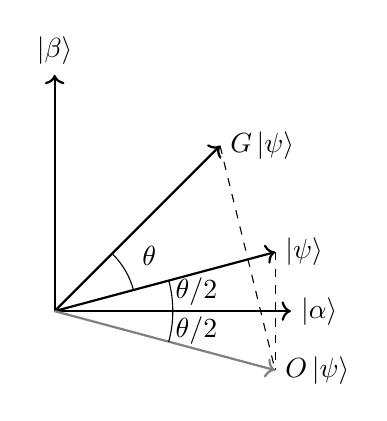
\begin{tikzpicture}
        % 绘制箭头
        \draw[->, thick] (0,0) -- (0,3) node[anchor=south] {$\ket{\beta}$};
        \draw[->, thick] (0,0) -- (2.1,2.1) node[anchor=west] {$G\ket{\psi}$};
        \draw[->, thick] (0,0) -- (2.8,0.75) node[anchor=west] {$\ket{\psi}$};
        \draw[->, thick] (0,0) -- (3,0) node[anchor=west] {$\ket{\alpha}$};
        \draw[->, gray, thick] (0,0) -- (2.8,-0.75) node[anchor=west,black] {$O\ket{\psi}$};
        % 绘制虚线
        \draw[dashed] (2.8,0.75) -- (2.8,-0.75);
        \draw[dashed] (2.1,2.1) -- (2.8,-0.75);
        % 绘制角度标记
        \draw (1.5,0) arc[start angle=0,end angle=15,radius=1.5];
        \draw (1.5,0) arc[start angle=0,end angle=-15,radius=1.5];
        \draw (1,0.27) arc[start angle=15,end angle=45,radius=1];
        % 标记角度
        \node at (1.8,0.25) {$\theta/2$};
        \node at (1.8,-0.25) {$\theta/2$};
        \node at (1.2,0.7) {$\theta$};
    \end{tikzpicture}
    \caption{}
    \label{fig:grover}
\end{figure}

Let $\sin(\theta/2)=\sqrt{M/N}$,  the angle between $\ket{\psi}$ and $\ket{\alpha}$ is $\theta/2$. As shown in Figure \ref{fig:grover},  operation $G=WO$ gives us a rotation of angle $\theta$, we call $G$ the Grover iteration. So we just need applying $R\coloneqq\left\lfloor\frac{\pi-\theta}{2\theta}\right\rceil$\footnote{The actual function about $\left\lfloor x\right\rceil$ is to denote the integer closest to the real number $x$.} times Grover iteration on $\ket{\psi}$ to approximate $\ket{\beta}$, if $M\ll N$ we have
\begin{equation}
    G^{R}\ket{\psi}=\cos(\frac{2R+1}{2}\theta)\ket{\alpha}+\sin(\frac{2R+1}{2}\theta)\ket{\beta}\approx\ket{\beta}.
\end{equation}
The angular error is at most $\theta/2\approx\sqrt{M/N}$.



\subsection{Oracle}

Let's construct the reflection about $\ket{\alpha}$, we call it the oracle. We know that states in the space spanned by $\ket{\alpha}$ and $\ket{\beta}$ can be decomposed into
\begin{equation}
    \ket{x}=\ket{\alpha}\braket{\alpha|x}+\ket{\beta}\braket{\beta|x}
\end{equation}
and we wish
\begin{equation}
    O\ket{x}=\ket{\alpha}\braket{\alpha|x}-\ket{\beta}\braket{\beta|x}.
\end{equation}
But we don't know the exact form of $\ket{\alpha}$ and $\ket{\beta}$. To construct this, we need a special gate\footnote{Note that the mapping $\ket{x}\xrightarrow{U_{f}}(-1)^{f(x)}\ket{x}$ holds only if the controlled qubit is $\ket{-}$.}
\begin{equation}
    \begin{quantikz}
        \lstick{$\ket{x}$} & \qwbundle{n} & \gate[2][1.7cm]{U_{f}}\gateinput{$x$}\gateoutput{$x$} & \rstick{$(-1)^{f(x)}\ket{x}$} \\
        \lstick{$\ket{-}$} & & \gateinput{$y$}\gateoutput{$y\oplus f(x)$} & \rstick{$\ket{-}$}
    \end{quantikz}
\end{equation}
which gives us a operation $\ket{x}\xrightarrow{U_{f}}(-1)^{f(x)}\ket{x}$. Then we just need to construct the mapping
\begin{equation}
    S(x)=
    \begin{cases}
        1 & x\in T    \\
        0 & x\notin T
    \end{cases}
\end{equation}
such that $U_{S}$ satisfies the properties we need:
\begin{equation}
    \begin{split}
        U_{S}\ket{\beta}  & =-\ket{\beta}  \\
        U_{S}\ket{\alpha} & =\ket{\alpha}.
    \end{split}
\end{equation}
So the $U_{S}$ is the Oracle.



\subsection{Grover iteration}

Then, let's construct the reflection about $\ket{\psi}$. Same as the oracle, we decompose states into
\begin{equation}
    \ket{x}=\ket{\psi}\braket{\psi|x}+\ket{\psi_{\perp}}\braket{\psi_{\perp}|x}
\end{equation}
which $\ket{\psi_{\perp}}=\sqrt{\frac{M}{N}}\ket{\alpha}-\sqrt{\frac{N-M}{N}}\ket{\beta}$, and we wish
\begin{equation}
    W\ket{x}=\ket{\psi}\braket{\psi|x}-\ket{\psi_{\perp}}\braket{\psi_{\perp}|x}.
\end{equation}
But this time, we know $\ket{\psi}$ specifically. Operation $2\ket{\psi}\bra{\psi}-I$ is what we need which satisfies the properties:
\begin{equation}
    \begin{split}
        (2\ket{\psi}\bra{\psi}-I)\ket{\psi}         & =\ket{\psi}           \\
        (2\ket{\psi}\bra{\psi}-I)\ket{\psi_{\perp}} & =-\ket{\psi_{\perp}}.
    \end{split}
\end{equation}
So we get the construction of the Grover iteration:
\begin{equation}
    G=WO=(2\ket{\psi}\bra{\psi}-I)U_{S}.
\end{equation}
After constructing each sub-operation, the circuit of the algorithm is given here\footnote{The oracle workspace is omitted here.}:
\begin{equation}
    \begin{quantikz}[column sep=0.4cm]
        \lstick{$\ket{0}$} & \qwbundle{n} & \gate{H^{\otimes n}} & \gate[2]{oracle}\gategroup[wires=2,steps=4]{Grover iteration} & \gate{H^{\otimes n}} & \gate{2\ket{0}\bra{0}-I} & \gate{H^{\otimes n}} & \gate[2]{G} & \midstick[2,brackets=none]{$\cdots$} & \gate[2]{G} & \\
        \lstick{$\ket{1}$} & & \gate{H} & & & & & & & &
    \end{quantikz}
\end{equation}
The ellipsis indicates that it is repeated $R$ times.



\subsection{Performance}

Each of the operations in the Grover iteration may be efficiently implemented on a quantum computer. So we just need to focus on the number of Grover iterations.

We already know, in order to rotate $\ket{\psi}$ near $\ket{\beta}$, we need to repeat the Grover iteration
\begin{equation}
    R=\left\lfloor\frac{2\arccos\sqrt{M/N}}{\arcsin\sqrt{M/N}}\right\rceil
\end{equation}
times. This is not intuitive enough, so let's sacrifice some precision to find a simpler expression. We know that $R\leq\left\lceil\pi/2\theta\right\rceil$, and if $M\leq N/2$ we have
\begin{equation}
    \frac{\theta}{2}\geq\sin\frac{\theta}{2}=\sqrt{\frac{N}{M}},
\end{equation}
from which we obtain an elegant upper bound on the number of iterations required,
\begin{equation}
    R\leq\left\lceil\frac{\pi}{4}\sqrt{\frac{N}{M}}\right\rceil.
\end{equation}
That is, $R=O(\sqrt{N/M})$ Grover iterations must be performed to obtain a solution to the search problem with high probability, a quadratic improvement over the $O(N/M)$oracle calls required classically.

If $M>N/2$, the quantum search algorithm is not necessary. We can just randomly pick an item from the search space, and then check that it is a solution using the oracle. This approach has a success probability of at least one-half and only requires one consultation with the oracle.



\section{Bounds for Grover's algorithm}

\textit{This section is based on the paper\cite{2009Exact}.}

\subsection{Main idea}

Oracle is at the heart of Grover's algorithm, so let's focus on the oracle and ignore the other operations, we write the state that uses $R$ queries to the oracle as
\begin{equation}
    \ket{\Psi_{x}^{R}}=\prod_{j=1}^{R}U_{j}O_{x}\ket{\psi},
\end{equation}
where $U_{i}$ is some unitary operation and $O_{x}$ is the oracle which marks the target element $x$. To illustrate the effect of oracles, let's replace some of them with unit operations, we write
\begin{equation}
    \ket{\Psi_{x}^{i,R}}=\prod_{j=i+1}^{R}U_{j}O_{x}\prod_{j=1}^{i}U_{j}I\ket{\psi},
\end{equation}
which uses the identity for the first $i$ oracle queries and the oracle for the latter $R-i$ oracle queries. If there is no application oracle,  then the state is independent of the target element and may be denoted as
\begin{equation}
    \ket{\Psi^{R}}=\prod_{j=1}^{R}U_{j}I\ket{\psi}.
\end{equation}
So that we can find the distance changed by oracle, here we use two kinds of metric, euclidean distance and angular distance:
\begin{equation}
    E(\ket{\alpha},\ket{\beta})=\left\|\ket{\alpha}-\ket{\beta}\right\|
    \quad\text{and}\quad
    A(\ket{\alpha},\ket{\beta})=\arccos\frac{\left\lvert \braket{\alpha|\beta}\right\rvert}{\left\|\ket{\alpha}\right\|\left\|\ket{\beta}\right\|}.
\end{equation}
Taking the distance $E$ as an example, if $\Psi_{x}^{R}$ satisfies the properties the output should have
\begin{equation}\label{TheOutputWeWant}
    \left\| \mathsf{\Pi}_{x}\ket{\Psi_{x}^{R}} \right\|^{2} \geq p
\end{equation}
which $\{\mathsf{\Pi}_{j}\}$ is a finite set of orthogonal projectors that sum to the identity and $p$ is the probability we want of outputting the correct element.

We can calculate the number of queries $R$ by dividing $E(\ket{\Psi_{x}^{R}},\ket{\Psi^{R}})$ with the distance changed by oracle\footnote{Note that this is just a loose intuition, which we'll prove in the next subsection.}, that is
\begin{equation}\label{TheNumberForIteration}
    R=\frac{E(\ket{\Psi_{x}^{R}},\ket{\Psi^{R}})}{E(O_{x}\ket{\gamma},\ket{\gamma})}.
\end{equation}
It is important to note that $\ket{\gamma}$ here is not some particular state, we will calculate the mean of the distance changed by oracle on each state.



\subsection{\label{DistanceByOracle}Distance the oracle changes}

First, let's calculate the distance changed by the oracle. Considering the distance of the state before and after $R$ oracle queries, we have
\begin{lemma}
    The average \textcolor{red}{euclidean distance} after $R$ oracle queries is at most
    \begin{equation}
        \frac{1}{N}\sum_{x=1}^{N}\textcolor{red}{E}(\ket{\Psi_{x}^{R}},\ket{\Psi^{R}})\leq 2R\textcolor{red}{\frac{1}{\sqrt{N}}}.
    \end{equation}
\end{lemma}
\begin{proof}
    With triangle inequality,
    \begin{equation*}
        \begin{split}
            \frac{1}{N}\sum_{x=1}^{N}\textcolor{red}{E}(\ket{\Psi_{x}^{R}},\ket{\Psi^{R}})
             & = \frac{1}{N}\sum_{x=1}^{N}\textcolor{red}{E}(\ket{\Psi_{x}^{0,R}},\ket{\Psi_{x}^{R,R}})
            \leq \frac{1}{N}\sum_{x=1}^{N}\sum_{i=1}^{R}\textcolor{red}{E}(\ket{\Psi_{x}^{i-1,R}},\ket{\Psi_{x}^{i,R}}) \\
             & = \frac{1}{N}\sum_{i=1}^{R}\sum_{x=1}^{N}\textcolor{red}{E}(O_{x}\ket{\Psi^{i}},\ket{\Psi^{i}})
            = \frac{1}{N}\sum_{i=1}^{R}\sum_{x=1}^{N}\textcolor{red}{2\left\|\mathsf{\Pi}_{x}\ket{\Psi^{i}}\right\|}    \\
             & \leq 2\sum_{i=1}^{R}\textcolor{red}{\frac{1}{\sqrt{N}}} = 2R\textcolor{red}{\frac{1}{\sqrt{N}}},
        \end{split}
    \end{equation*}
    where the last inequality that needs to be noticed is that
    \begin{equation}\label{Cauchy-Schwarz}
        \left(\sum_{i=1}^{N}a_{i}\right)^{2}=\sum_{i=1}^{N}a_{i}^{2}+2\sum_{i=1}^{N}\sum_{j=1}^{i-1}a_{i}a_{j}\leq N\sum_{i=1}^{N}a_{i}^{2},
    \end{equation}
    that is
    \begin{equation*}
        \sum_{x=1}^{N}\frac{1}{N}\left\|\mathsf{\Pi}_{x}\ket{\Psi^{i}}\right\|\leq \sqrt{\frac{1}{N}\sum_{x=1}^{N}\left\|\mathsf{\Pi}_{x}\ket{\Psi^{i}}\right\|^{2}}=\frac{1}{\sqrt{N}}. \qedhere
    \end{equation*}
\end{proof}
\begin{lemma}
    The average \textcolor{blue}{angular distance} after $R$ oracle queries is at most
    \begin{equation}
        \frac{1}{N}\sum_{x=1}^{N}\textcolor{blue}{A}(\ket{\Psi_{x}^{R}},\ket{\Psi^{R}})\leq 2R\textcolor{blue}{\arcsin(\frac{1}{\sqrt{N}})}.
    \end{equation}
\end{lemma}
\begin{proof}
    With triangle inequality,
    \begin{equation*}
        \begin{split}
            \frac{1}{N}\sum_{x=1}^{N}\textcolor{blue}{A}(\ket{\Psi_{x}^{R}},\ket{\Psi^{R}})
             & = \frac{1}{N}\sum_{x=1}^{N}\textcolor{blue}{A}(\ket{\Psi_{x}^{0,R}},\ket{\Psi_{x}^{R,R}})
            \leq \frac{1}{N}\sum_{x=1}^{N}\sum_{i=1}^{R}\textcolor{blue}{A}(\ket{\Psi_{x}^{i-1,R}},\ket{\Psi_{x}^{i,R}})           \\
             & = \frac{1}{N}\sum_{i=1}^{R}\sum_{x=1}^{N}\textcolor{blue}{A}(O_{x}\ket{\Psi^{i}},\ket{\Psi^{i}})
            = \frac{1}{N}\sum_{i=1}^{R}\sum_{x=1}^{N}\textcolor{blue}{\arccos(\left\lvert\cos(2\theta_{x}^{i})\right\rvert)}       \\
             & \leq 2\sum_{i=1}^{R}\textcolor{blue}{\arcsin(\frac{1}{\sqrt{N}})} = 2R\textcolor{blue}{arcsin(\frac{1}{\sqrt{N}})},
        \end{split}
    \end{equation*}
    where has $\theta_{x}^{i}=A(\ket{\Psi^{i}},\ket{x_{\perp}})=\arcsin\left\| \mathsf{\Pi}_{x}\ket{\Psi^{i}}\right\|$. And where the last inequality still needs to notice the rescaling provided by equation \ref{Cauchy-Schwarz}, that is
    \begin{equation*}
        \sum_{x=1}^{N}\frac{1}{N}\arcsin\left\|\mathsf{\Pi}_{x}\ket{\Psi^{i}}\right\|\leq\arcsin\sum_{x=1}^{N}\frac{1}{N}\left\|\mathsf{\Pi}_{x}\ket{\Psi^{i}}\right\|\leq\arcsin\frac{1}{\sqrt{N}},
    \end{equation*}
    where also need notice that $\sum_{x=1}^{N}\frac{1}{N}\arcsin a_{i}\leq\arcsin\sum_{x=1}^{N}\frac{1}{N}a_{i}$ which $a_{i}\in\left[0,\frac{\pi}{2}\right]$.
\end{proof}
According to the theorem, the distance changed by each oracle query can only add up linearly.



\subsection{\label{DistanceWhenWeNeed}Distance when the output is we need}

Then, let's calculate the distance when equation \ref{TheOutputWeWant} is satisfied.
\begin{lemma}
    Suppose that the algorithm correctly outputs $y$ with probability at least $p$ after $R$ queries, given oracle $O_{y}$. Then the average Euclidean distance is at least
    \begin{equation}
        \frac{1}{N}\sum_{x=1}^{N}E(\ket{\Psi_{x}^{R}},\ket{\Psi^{R}})\geq \frac{1}{\sqrt{2}}\left(\sqrt{p}-\sqrt{1-p}+1-\frac{2}{\sqrt{N}}\right).
    \end{equation}
\end{lemma}
\begin{proof}
    For a certain $x$, we have
    \begin{equation*}
        \begin{split}
            E(\ket{\Psi_{x}^{R}},\ket{\Psi^{R}})
             & \geq \frac{1}{\sqrt{2}}\left(\left\|\mathsf{\Pi}_{x}\left(\ket{\Psi_{x}^{R}}-\ket{\Psi^{R}}\right)\right\|+\left\|\mathsf{\Pi}_{x}^{\perp}\left(\ket{\Psi_{x}^{R}}-\ket{\Psi^{R}}\right)\right\|\right)                                             \\
             & \geq \frac{1}{\sqrt{2}}\left(\left\|\mathsf{\Pi}_{x}\ket{\Psi_{x}^{R}}\right\|-\left\|\mathsf{\Pi}_{x}\ket{\Psi^{R}}\right\|+\left\|\mathsf{\Pi}_{x}^{\perp}\ket{\Psi^{R}}\right\|-\left\|\mathsf{\Pi}_{x}^{\perp}\ket{\Psi_{x}^{R}}\right\|\right) \\
             & \geq \frac{1}{\sqrt{2}}\left(\left\|\mathsf{\Pi}_{x}\ket{\Psi_{x}^{R}}\right\|-\left\|\mathsf{\Pi}_{x}^{\perp}\ket{\Psi_{x}^{R}}\right\|+1-2\left\|\mathsf{\Pi}_{x}\ket{\Psi^{R}}\right\|\right)                                                    \\
             & \geq \frac{1}{\sqrt{2}}\left(\sqrt{p}-\sqrt{1-p}+1-2\left\|\mathsf{\Pi}_{x}\ket{\Psi^{R}}\right\|\right),
        \end{split}
    \end{equation*}
    where the last inequality from the success probability is at least $p$. To eliminate the last term, consider a traversal of $x$
    \begin{equation*}
        \frac{1}{N}\sum_{x=1}^{N}E(\ket{\Psi_{x}^{R}},\ket{\Psi^{R}})
        \geq \frac{1}{\sqrt{2}}\left(\sqrt{p}-\sqrt{1-p}+1-\frac{2}{N}\sum_{x=1}^{N}\left\|\mathsf{\Pi}_{x}\ket{\Psi^{R}}\right\|\right)
        \geq \frac{1}{\sqrt{2}}\left(\sqrt{p}-\sqrt{1-p}+1-\frac{2}{\sqrt{N}}\right),
    \end{equation*}
    where the last inequality uses the equation \ref{Cauchy-Schwarz} again.
\end{proof}
\begin{lemma}
    Suppose that the algorithm correctly outputs $y$ with probability at least $p$ after $R$ queries, given oracle $O_{y}$. Then the average angular distance is at least
    \begin{equation}
        \frac{1}{N}\sum_{x=1}^{N}A(\ket{\Psi_{x}^{R}},\ket{\Psi^{R}})\geq \arcsin\sqrt{p}-\arcsin\frac{1}{\sqrt{N}}.
    \end{equation}
\end{lemma}
\begin{proof}
    For a certain $x$, we have
    \begin{equation*}
        \begin{split}
            A(\ket{\Psi_{x}^{R}},\ket{\Psi^{R}})
             & = \arccos\left(\left\lvert \braket{\Psi_{x}^{R}|\Psi^{R}}\right\rvert\right)                                                                                                                                                                  \\
             & = \arccos\left(\bra{\Psi_{x}^{R}}(\mathsf{\Pi}_{x}+\mathsf{\Pi}_{x}^{\perp})^{\dagger}(\mathsf{\Pi}_{x}+\mathsf{\Pi}_{x}^{\perp})\ket{\Psi^{R}}\right)                                                                                        \\
             & = \arccos\left(\left\|\mathsf{\Pi}_{x}\ket{\Psi_{x}^{R}}\right\|\cdot\left\|\mathsf{\Pi}_{x}\ket{\Psi^{R}}\right\|+\left\|\mathsf{\Pi}_{x}^{\perp}\ket{\Psi_{x}^{R}}\right\|\cdot\left\|\mathsf{\Pi}_{x}^{\perp}\ket{\Psi^{R}}\right\|\right) \\
             & = \arccos\left(\sin\phi_{x}^{R}\sin\theta_{x}^{R}+\cos\phi_{x}^{R}\cos\theta_{x}^{R}\right)                                                                                                                                                   \\
             & = \phi_{x}^{R}-\theta_{x}^{R} \geq \arcsin\sqrt{p}-\theta_{x}^{R},
        \end{split}
    \end{equation*}
    where has $\phi_{x}^{i}=\arcsin\left\| \mathsf{\Pi}_{x}\ket{\Psi_{x}^{i}}\right\|$ and still has $\theta_{x}^{i}=\arcsin\left\| \mathsf{\Pi}_{x}\ket{\Psi^{i}}\right\|$, and where the last inequality from the success probability being at least $p$. Just like the last proof, consider a traversal of $x$
    \begin{equation*}
        \frac{1}{N}\sum_{x=1}^{N}A(\ket{\Psi_{x}^{R}},\ket{\Psi^{R}})
        \geq \arcsin\sqrt{p}-\frac{1}{N}\sum_{x=1}^{N}\theta_{x}^{R}
        \geq \arcsin\sqrt{p}-\arcsin\frac{1}{\sqrt{N}},
    \end{equation*}
    where the last inequality uses the equation \ref{Cauchy-Schwarz} again.
\end{proof}



\subsection{Lower bound of Grover iterations}



From section \ref{DistanceByOracle} and section \ref{DistanceWhenWeNeed}, we obtain the two parts required for equation \ref{TheNumberForIteration} to compute the number of iterations: the upper bound of the distance changed by oracle and the lower bound of the distance when the output is we need. So we have the lower bound on the number of iterations for both versions
\begin{theorem}
    The unordered search problem with success probability $p>0$ requires at least $R$ queries, where
    \begin{equation}
        R =\frac{\sqrt{N}}{2\sqrt{2}}\left(\sqrt{p}-\sqrt{1-p}+1-\frac{2}{\sqrt{N}}\right).
    \end{equation}
\end{theorem}
\begin{theorem}
    The unordered search problem with success probability $p>0$ requires at least $R$ queries, where
    \begin{equation}
        R =\frac{\arcsin\sqrt{p}-\arcsin\frac{1}{\sqrt{N}}}{2\arcsin\frac{1}{\sqrt{N}}}.
    \end{equation}
\end{theorem}
In the case of Euclidean distances, we conclude that Grover's algorithm is asymptotically optimal, and in the case of angular distances, Grover's algorithm is exactly optimal.



\section{Long algorithm}

\textit{This section is based on the paper\cite{Long_2001}.}

\subsection{\label{subsec:LongMainIdea}Main idea}

Although Grover's algorithm is already accurate enough when the number of elements is large, for instance in deciphering the DES code where $N = 256$ the deviation is only $3\times 10^{-9}$. But in problems where certainly is vital, especially when the dimension is not so big, using a searching algorithm with certainty becomes important. Let's make some improvements to the Grover's algorithm.

In the Grover's algorithm\footnote{The notation of section \ref{subsec:GroverMainIdea} is followed here.} we construct rotations in the space spanned by $\ket{\alpha}$ and $\ket{\beta}$, but $SU(2)$ has three degrees of freedom, so we may as well extend $G=WO=(I-2\ket{\psi_{\perp}}\bra{\psi_{\perp}})(I-2\ket{\beta}\bra{\beta})$ to
\begin{equation}
    \begin{split}
        I_{W} & = I+(e^{-i\phi}-1)\ket{\psi_{\perp}}\bra{\psi_{\perp}} = e^{-i\phi}(I+(e^{i\phi}-1)\ket{\psi}\bra{\psi})                   \\
        I_{O} & = I+(e^{i\phi}-1)\ket{\beta}\bra{\beta}                                                                                    \\
        Q     & = I_{W}I_{O} = e^{-i\phi}H^{\otimes n}(I+(e^{i\phi}-1)\ket{0}\bra{0})H^{\otimes n}(I+(e^{i\phi}-1)\ket{\beta}\bra{\beta}).
    \end{split}
\end{equation}
Intuitively, if we want $Q$ to make $\ket{\psi}$ go to $\ket{\beta}$, we should have the axis of rotation at the same angle as $\ket{\psi}$ and $\ket{\beta}$. From corollary \ref{cor:CompositionOfRotation}, if the angle of $I_{O}$ is $-\phi$, the angle of $I_{W}$ has to be $\phi$. As a generalization of Grover's algorithm, it can be seen that if we set $\phi=\pi$, then $Q$ degenerates to $G$.
\begin{figure}[h]
    \centering
    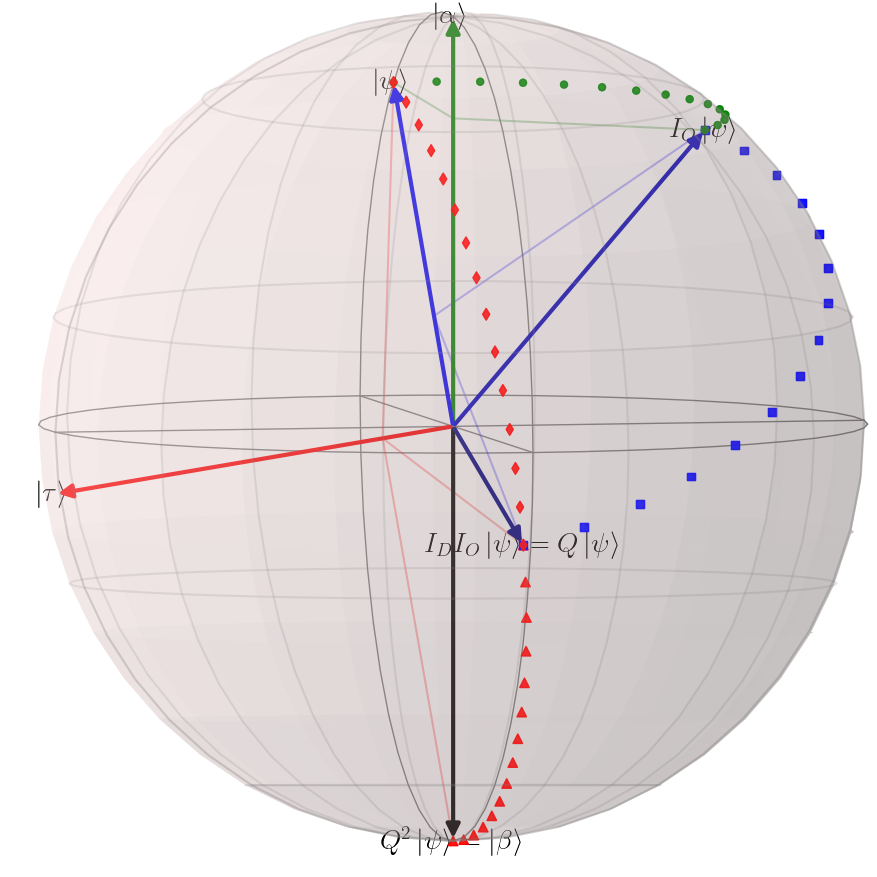
\includegraphics[width=0.5\columnwidth]{figures/long.png}
    \caption{}
    \label{fig:long}
\end{figure}

As shown in the Figure \ref{fig:long}, $I_{O}$ gives us a rotation of angle $-\phi$ about axis $\vec{r}_{\alpha}=(0,0,1)^{T}$ and $I_{W}$ gives us a rotation of angle $\phi$ about axis $\vec{r}_{\psi}=(\sin\theta,0,\cos\theta)^{T}$, their product $Q=I_{W}I_{O}$ gives us a rotation of angle
\begin{equation}
    \omega=4\arcsin(\sin\frac{\phi}{2}\sin\frac{\theta}{2})
\end{equation}
about axis
\begin{equation}
    \vec{r}_{q}= k(\cos\frac{\phi}{2},\sin\frac{\phi}{2},\cos\frac{\phi}{2}\tan\frac{\theta}{2})^{T},
\end{equation}
where $k$ is the normalization factor.

A naive thought is whether we can find a suitable $\phi$ such that $\ket{\psi}$ can turn to $\ket{\beta}$ exactly. The angle we need to rotate about axis $\ket{q}$ is
\begin{equation}\label{eq:LongDeltaAngle}
    e^{i\Delta\varphi}=\frac{\braket{q_{\perp}|\beta}}{\braket{q_{\perp}|\psi}},
\end{equation}
we wish $j=\frac{\Delta\varphi}{\omega}$ is an integer, so that we have $Q^{j}\ket{\psi}=\ket{\beta}$.

\subsection{The right angle\label{subsec:RightAngle}}

Using equation \ref{eq:LongDeltaAngle} to calculate the angle $\Delta\varphi$ is complicated, so we may as well calculate it with Bloch vectors.
\begin{figure}[h]
    \centering
    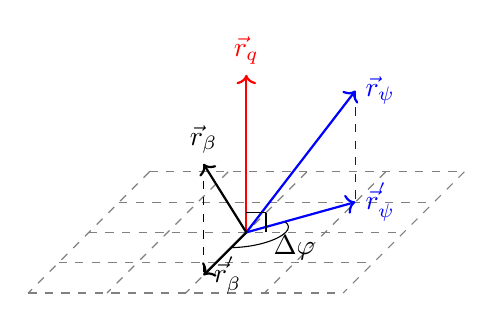
\begin{tikzpicture}
        % grid
        \draw[dashed, gray] (-2,0,-2) -- (2,0,-2);
        \draw[dashed, gray] (-2,0,-1) -- (2,0,-1);
        \draw[dashed, gray] (-2,0,0) -- (2,0,0);
        \draw[dashed, gray] (-2,0,1) -- (2,0,1);
        \draw[dashed, gray] (-2,0,2) -- (2,0,2);
        \draw[dashed, gray] (-2,0,-2) -- (-2,0,2);
        \draw[dashed, gray] (-1,0,-2) -- (-1,0,2);
        \draw[dashed, gray] (0,0,-2) -- (0,0,2);
        \draw[dashed, gray] (1,0,-2) -- (1,0,2);
        \draw[dashed, gray] (2,0,-2) -- (2,0,2);

        % vectors
        \draw[->, thick, red] (0,0,0) -- (0,2,0) node[anchor=south]{$\vec{r}_q$};% q
        \draw[->, thick, blue] (0,0,0) -- (1,1.414,-1) node[anchor=west]{$\vec{r}_\psi$};% psi
        \draw[->, thick, blue] (0,0,0) -- (1,0,-1) node[anchor=west]{$\vec{r}_\psi^{'}$};% psi_aux
        \draw[->, thick, black] (0,0,0) -- (0,1.414,1.414) node[anchor=south]{$\vec{r}_\beta$};% beta
        \draw[->, thick, black] (0,0,0) -- (0,0,1.414) node[anchor=west]{$\vec{r}_\beta^{'}$};% beta_aux

        % perp
        \draw[thin, black] (0,0.25,0) -- (0.25,0.25,0);
        \draw[thin, black] (0.25,0,0) -- (0.25,0.25,0);

        % lines
        \draw[dashed, blue] (1,1.414,-1) -- (1,0,-1);
        \draw[dashed, black] (0,1.414,1.414) -- (0,0,1.414);

        % angles
        \draw[canvas is xz plane at y=0] (0.353,-0.353) arc[start angle=-45,end angle=90,radius=0.5];

        % angles label
        \node at (0.8,0,0.5) {$\Delta\varphi$};
    \end{tikzpicture}
    \caption{}
    \label{fig:AuxLong}
\end{figure}

As shown in the Figure \ref{fig:AuxLong}, we can calculate the angle between the projections of $\vec{r}_{\psi}$ and $\vec{r}_{\beta}$ on the plane perpendicular to $\vec{r}_{q}$, we call these projections
\begin{equation}
    \begin{split}
        \vec{r}_{\psi}^{'}  & =\vec{r}_{\psi}-(\vec{r}_{\psi}\cdot\vec{r}_{q})\vec{r}_{q}    \\
        \vec{r}_{\beta}^{'} & =\vec{r}_{\beta}-(\vec{r}_{\beta}\cdot\vec{r}_{q})\vec{r}_{q},
    \end{split}
\end{equation}
so that we can express $\Delta\varphi$ in a simpler form
\begin{equation}
    \Delta\varphi=\arccos\frac{\vec{r}_{\psi}^{'}\cdot\vec{r}_{\beta}^{'}}{\|\vec{r}_{\psi}^{'}\|\|\vec{r}_{\beta}^{'}\|}.
\end{equation}
After some boring calculations, we can get
\begin{equation}
    \Delta\varphi=2\arccos(\sin\frac{\phi}{2}\sin\frac{\theta}{2}).
\end{equation}

After calculating each part we need, let's find the right angle $\phi$! Though section \ref{subsec:LongMainIdea}, The iterations $j=\frac{\Delta\varphi}{\omega}$ must be an integer. For equation $\Delta\varphi=j\omega$, consider both ends of the equation separately, we have
\begin{equation}
    \begin{split}
        \Delta\varphi & = 2\arccos(\sin\frac{\phi}{2}\sin\frac{\theta}{2})                            \\
                      & = 2\left(\frac{\pi}{2}-\arcsin(\sin\frac{\phi}{2}\sin\frac{\theta}{2})\right) \\
        j\omega       & = 4j\arcsin(\sin\frac{\phi}{2}\sin\frac{\theta}{2}),
    \end{split}
\end{equation}
so that we have
\begin{equation}
    \sin\frac{\phi}{2} = \frac{\sin\left(\frac{\pi}{4j+2}\right)}{\sin\frac{\theta}{2}},
\end{equation}
notice that $\phi$ has a real solution only when $\theta/2\geq\pi/(4j+2)$, may as well let $j=\left\lceil(\pi-\theta)/(2\theta) \right\rceil$, so we worked out the right angle $\phi$
\begin{equation}
    \phi=2\arcsin\left(\frac{\sin\left(\frac{\pi}{4j+2}\right)}{\sin\frac{\theta}{2}}\right).
\end{equation}

Let's finish with some examples of $j$ and $\phi$:
\begin{table}[h!]
    \centering
    \begin{equation*}
        \begin{array}{ccccccccccc}
            \toprule
            N        & 2   & 4 & 8        & 100      & 1000     & 10^{4}   & 10^{6}  & 10^{8}   & 10^{10}  & 2^{56} \\
            \midrule
            j        & 1   & 1 & 2        & 3        & 8        & 25       & 79      & 785      & 7854     & 78540  \\
            \phi/\pi & 0.5 & 1 & 0.677007 & 0.698709 & 0.748018 & 0.854022 & 0.90089 & 0.989752 & 0.992688 & 0.9973 \\
            \bottomrule
        \end{array}
    \end{equation*}
    \caption{}
    \label{tab:examples}
\end{table}

Can be seen as $N$ increases, the angle $\phi$ approaches $\pi$. At this point, Long's algorithm is also slightly closer to Grover's algorithm.



%-----------------------bib---------------------------

\bibliographystyle{plain}
\bibliography{ref}


\end{document}